\documentclass[11pt,a4paper]{article}
\usepackage[margin=2.3cm]{geometry}
\usepackage{amsmath,amssymb,graphicx,booktabs,hyperref,caption}
\captionsetup{font=small}
% numbers and result paragraphs; sources: study/insitu/out/server/*.json, docs/CRITIC_INSITU_1.md
\newcommand{\nknotimg}{124}
\newcommand{\splineerr}{0.19}
\newcommand{\gradspeedA}{10}
\newcommand{\iterspeedA}{5}
\newcommand{\breakevenA}{300}
\newcommand{\nseeds}{3}
\newcommand{\gpu}{RTX 3090}
\newcommand{\nbench}{16{,}000}

\newcommand{\speedtext}{%
At that setting the pupil model costs 23\,$\mu$s per emitter and the spline 2.3\,$\mu$s; the fixed cost of the
knot route (one build of the knots that keeps the computation graph, and one backward pass) is 7\,ms. The
gradient is cheaper from about 320 emitters on, 7.6 times at $10^4$ and 10 times at $10^5$ emitters and above.
Re-localizing the emitters costs another 2.5\,$\mu$s per emitter in both routes, so a whole iteration is 5.0 to
5.3 times cheaper. With the coarser 64/3 setting, whose error (0.39\,\%) is twice that of the spline, the
numbers are 4 (gradient) and 2.5 (iteration); a complete fit of 16{,}000 emitters, 40 iterations, took 5.3\,s
through the knots and 8.9\,s per emitter, and both ended at the same Zernike error (Fig.~\ref{fig:speed},
right). The 256/6 setting gives a factor 46 for the gradient at $10^5$ emitters, but that pupil model is ten
times more accurate than the spline it is compared with, so this row is not a like-for-like comparison.}

\newcommand{\gradtext}{%
At the starting point of a fit (Zernikes from the bead stack, or the truth plus 0.01 waves) the two gradients
agree to 0.2\,\% (cosine similarity 1.000000). Near the optimum the gradient is small, and the interpolation
error of the spline becomes visible: at the true parameters the two routes differ by 4\,\% for the Zernikes, 4\,\%
for a pupil phase map and 12\,\% for a pupil amplitude map (measured by the reviewer of this study,
\texttt{critic/grad\_speed.py}, 2000 emitters). On noise-free data this moves the optimum of the Zernike
coefficients by $1.6\times10^{-5}$ waves rms. That is far below any physical relevance, but it is the size of
the statistical error at about $10^6$ emitters, so beyond that a finer spline ($S=3$) or a final step with the
per-emitter route would be needed. In the fits of this study the Zernike error at convergence is set by the
difference between the simulated and the fitted pupil sampling ($5$--$8\times10^{-4}$ waves in scenario A).}

\newcommand{\acctext}{%
Table~\ref{tab:acc} and Fig.~\ref{fig:bias}.

\emph{Beads only.} With the aberration change chosen here, a PSF from the bead stack alone is far off on the
sample data: 15--18 nats per emitter, z errors of 65--80\,nm rms, and for the Zernike model a y error that
changes by 120--180\,nm over the z range. This is a statement about the chosen aberration change, not a general
one, and the bead spline uses the paraxial depth scaling without the empirical correction that is common
practice.

\emph{Scenario A.} The Zernike model refined on the movie patches, starting from the bead fit, is
indistinguishable from the true PSF in every column (8\,s for 11{,}600 patches). Free knots on top add noise
(z rms 22 to 27\,nm, a z-scale error of $-13\pm4$\,nm). A free pupil map on top changes nothing within the
spread over seeds.

\emph{Scenario B.} The refined Zernike model leaves a likelihood deficit of 2.7 nats per emitter, a y error
that grows by $45\pm1$\,nm over the z range, a z-scale error of $19\pm2$\,nm and a photon count that is 15\,\%
low. Free knots on top remove most of the deficit (0.22) and leave the y tilt ($43\pm1$\,nm), the z tilt and the
photon count where they were. This is the prediction of section~\ref{sec:gauge}: the three quantities that
blinking data do not determine stay at the values of the starting model. The free pupil map removes the deficit
(0.05), brings y and z precision to those of the true PSF, and reduces the y tilt to $8\pm5$\,nm on the movie
patches and $18\pm1$\,nm on clean patches; the photon count stays 9--10\,\% low. So the pupil physics removes
most of the z-dependent error but not all of it. Why the residual is larger on clean patches than on movie
patches was not investigated.

\emph{Shared spline.} A single free-knot spline fitted to beads and movie together fits the movie images
(deficit 0.2--0.3) but keeps the geometry of the bead stack: z offset 65\,nm, z-scale error of 75--107\,nm over
the range, photon counts 27--38\,\% low. A model-free spline is therefore not a usable in-situ PSF on its own
when the bead PSF and the sample PSF differ.

The movie gives few emitters at the top of the z range: the detection finds 57--67\,\% of the on-events below
500\,nm, 17\,\% at 600--700\,nm and 4\,\% at 700--800\,nm (Fig.~\ref{fig:zhist}), and the patches come from 700
sites, so they are not 11{,}600 independent emitters.}

\newcommand{\pitfalltext}{%
The spline stores the PSF on a support that allows emitter offsets up to $x_\text{max}$ from the patch centre,
and the localizer clamps the offset at that limit. In the first version of this study $x_\text{max}$ was
1.5 pixels. The patches are centred on the detection peak, and for a defocused, aberrated spot the peak is not
at the emitter: here it moves away by 1.2 pixels on average at 600--700\,nm height and by more than 3 pixels for
some spots. About 3\,\% of the patches then had the emitter beyond the limit, all at large z and on the same
side. The localizer could not reach them, and a flexible PSF model absorbed the difference: the free pupil map
showed a y tilt of 28--38\,nm in scenario A, where the Zernike start was already correct. The 17-term Zernike
model was too stiff to follow and stayed correct, which hid the problem. Controls located it: the same emitters
cropped at their true position gave no tilt, isolated emitters cropped at their detection peak gave 58\,nm, and
with $x_\text{max}=3$ pixels (all results above) the tilt is $1\pm3$\,nm. The independent review found the clamp
as the mechanism. The fraction of fitted emitters at the limit is now reported for every fit (below 0.1\,\%
here). Any localizer with a bounded offset has this failure mode when it is used inside a PSF estimation.}

\newcommand{\patterntext}{%
A lateral shift of the PSF with z is invisible in ordinary blinking data (section~\ref{sec:gauge}). A second,
PSF-independent measurement of the lateral position removes that freedom. We simulated emitters seen in 6
frames under a sinusoidal illumination pattern (2 orientations, 3 phases, pitch 220\,nm, modulation 0.9;
12{,}000 photons in total, 3000 emitters, clean patches); the emitter position is shared by the PSF term and the
pattern term of the likelihood. Table~\ref{tab:pattern}: with the pattern, the free pupil map in scenario B has
mean errors within $\pm1$\,nm in y and $\pm3$\,nm in z over the whole range, against a y error up to 14\,nm from
the same frames without pattern. Free knots lose their y error (44 to 2\,nm) but keep a z error of $-12$ to
$+21$\,nm: a lateral pattern says nothing about the labelling of the z axis.

This is a best case. The pattern (pitch, phases, modulation, registration to the camera) is taken as exactly
known, whereas in an experiment it is estimated from the same localizations; the emitters have three times the
photons of the movie; and the fit has to start from a PSF that is already roughly right (it first refines the
Zernikes on the summed frames), because from the bead PSF emitters lock onto the wrong fringe.}

\newcommand{\limittext}{%
\begin{itemize}\setlength\itemsep{0pt}
\item Simulation only. Data and fit share the vectorial model, NA, refractive indices, wavelength, dipole model
and Poisson noise; only the pupil sampling differs. A check by the reviewer with a sample index of 1.35 instead
of the 1.33 assumed by the fit gave a deficit of 0.10 nats and a z bias of $-22$ to $-5$\,nm for the Zernike
model: the optical constants have to be fitted or known.
\item Three seeds; the aberration change between beads and sample and the content of scenario B are single
arbitrary choices.
\item The speed comparison is between two routes in one code base on one GPU. No comparison with uiPSF or the
code of Droste et al.\ on the same data.
\item Field-constant PSF, uniform background, $15\times15$ patches, isolated spots only.
\item The regularization of the free-knot fits was chosen by looking at the test likelihood of scenario A.
\item The pattern experiment assumes a perfectly known pattern.
\item The settings where the speed matters most (field-dependent or time-dependent PSFs, very large data sets)
are not tested.
\end{itemize}}

\title{Differentiable spline for efficient in-situ estimation of point spread functions}
\author{Jelmer Cnossen}
\date{Draft, \today. Simulation study and a first test on real data.}
\begin{document}
\maketitle

\begin{abstract}
In 3D single-molecule localization microscopy the point spread function (PSF) of the sample differs from the PSF
measured on beads, so it has to be estimated from the blinking data itself (``in situ''). Maximum-likelihood
methods do this by evaluating a vectorial pupil model for every emitter in every iteration, which limits them to
a few thousand emitters. We separate the two costs. The pupil model is evaluated only on the knots of a cubic
spline (\nknotimg{} images), all emitters are evaluated on the spline, the likelihood gradient is summed on the
knots, and one backward pass through the pupil model turns it into the gradient for the pupil parameters. The
result equals the gradient of the per-emitter route up to the interpolation error of the spline. On simulated
astigmatic data the gradient is \gradspeedA{} times cheaper at $10^5$ emitters for a pupil model whose own
numerical error matches that of the spline, and a whole iteration (gradient plus re-localization) is
\iterspeedA{} times cheaper; below about \breakevenA{} emitters there is no gain. The same route fits a free
pixel map of pupil phase and amplitude. We also show which properties of a PSF blinking data cannot determine,
why a free-form spline PSF fitted in situ therefore keeps position errors that a pupil model does not, and
report an implementation pitfall (a limit on the fitted offset inside the patch) that biased flexible PSF models
in an earlier version of this study. On real astigmatic data of nuclear pores, refining a vectorial model in
situ through the knots improves the held-out likelihood over a bead-calibrated spline, but changes the
localization precision by 3\,\% at most and does not resolve the two rings of the pore; it does change the z
scale by about 10\,\%, and this data set cannot tell which z scale is right. On microtubule data the same
refinement again improves the likelihood without improving the precision, and the microtubule cross-section is
not a sharp enough ruler to settle the z scale. It does show that freely refined knots, which have by far the
best likelihood and the best frame-to-frame repeatability there, give wrong z positions.
\end{abstract}

\section{Introduction}

A 3D localization is only as accurate as the PSF model it is fitted with. The usual calibration, a z-stack of
beads on the coverslip, measures a different PSF from the one in the sample: the emitters sit at some depth in a
medium with a lower refractive index, and aberrations change between calibration and experiment. In-situ methods
estimate the PSF from the single-molecule data. INSPR~\cite{inspr} and VISPR~\cite{vispr} sort spots into z
classes, average them and run phase retrieval on the averages. uiPSF~\cite{uipsf} and the vectorial fit of
Droste et al.~\cite{droste} maximize the likelihood of all spots jointly over the PSF parameters and the emitter
parameters; both evaluate the pupil model for every emitter and report a few thousand emitters with run times
from half a minute (Zernike model on a CPU~\cite{droste}) to tens of minutes (field-dependent model on a
GPU~\cite{uipsf}).

Cubic-spline PSFs~\cite{cspline} are the standard for fast localization, because evaluating a spline costs far
less than evaluating a pupil model. Here the spline is used \emph{inside} the PSF estimation: as a layer between
the pupil model and the data that makes the cost of the pupil model independent of the number of emitters. The
questions of this study are (i) how much faster this is, and from how many emitters; (ii) whether the result is
the same; (iii) whether the spline knots themselves can serve as a free-form (``model-free'') in-situ PSF, and
when a pupil model with a few Zernike terms is not sufficient.

\section{Method}

\subsection{Spline PSF evaluated by a strided convolution}

The pixel-integrated PSF is taken as shift invariant within a patch: pixel $(i,j)$ of a $P\times P$ patch with
the emitter at offset $(x,y)$ from the patch centre and height $z$ has the expected value
$g(o_j-x,\;o_i-y,\;z)$, with $o$ the pixel offset from the centre. $g$ is stored as knots $c_{klm}$ on a grid
with spacing $1/S$ pixel laterally and $h_z$ axially, and interpolated with the Catmull--Rom cubic,
\begin{equation}
g(u,v,z)=\sum_{a,b,e=0}^{3} w_a(t_z)\,w_b(t_v)\,w_e(t_u)\;c_{k+a,\,l+b,\,m+e},
\end{equation}
where $(k,l,m)$ and $t\in[0,1)^3$ are the integer and fractional knot coordinates and $w(t)$ are the four cubic
weights. All pixels of a patch are $S$ knots apart and share the same $t$. A patch is therefore one
$4\times4\times4$ kernel applied to the knot array with stride $S$, and a batch of patches is one grouped
convolution. The derivatives with respect to $x,y,z$ use $w'(t)$ in one of the three factors. With $S=2$ and
$h_z=40$\,nm the spline differs from the pupil model it was built from by \splineerr\,\% (relative L2 norm).

\subsection{Implementation with a standard 2D convolution}
\label{sec:impl}

Spline PSFs for localization are usually stored as 64 polynomial coefficients per voxel and evaluated pixel by
pixel in a custom GPU kernel~\cite{cspline}. Here only the knot values are stored (one number per knot), and a
batch of patches is evaluated with operations that every deep-learning library already provides and has
optimized:
\begin{enumerate}\setlength\itemsep{0pt}
\item \emph{Weights.} For each emitter the fractional knot coordinates $t_u,t_v,t_z$ give three sets of four
cubic weights. Their outer product is one $4\times4\times4$ kernel per emitter.
\item \emph{Gather.} For each emitter a window of the knot array is read with one indexed gather: 4 planes in z
and $(P-1)S+4$ knots in each lateral direction ($32\times32$ for a $15\times15$ patch with $S=2$).
\item \emph{Convolution.} The windows of all $N$ emitters are stacked into one image with $4N$ channels and
passed through a single call of the 2D convolution of PyTorch (\texttt{conv2d}) with $N$ groups and stride $S$.
Each group holds one emitter: its four z planes are the input channels, its kernel is the $4\times4$ lateral
weights for each of them. The stride $S$ steps from one camera pixel to the next. The output is the
$N\times P\times P$ batch of patches.
\item \emph{Derivatives.} The derivatives with respect to $x$, $y$ and $z$ are three more output channels per
group, with $w'(t)$ in place of $w(t)$ in one factor. Value and derivatives come out of the same call.
\item \emph{Gradient on the knots.} Eq.~\eqref{eq:knotgrad} is the reverse pass of steps 2 and 3 (a transposed
convolution and a scatter-add), which automatic differentiation provides. No gradient code was written.
\end{enumerate}
The whole evaluation is about twenty lines of Python and has no custom kernel. It runs on any device PyTorch
supports, uses the vendor-optimized convolution, and can sit inside any other differentiable model, which is
what section~\ref{sec:passthrough} uses. Throughput is given in Table~\ref{tab:conv}. In the forward pass most of the time goes to building the indices and reading the knot windows; the convolution itself takes about a fifth. With the gradient, the backward pass of the convolution takes about two thirds and the read with its scatter-add one third (\texttt{bench\_split.py}). Storing knots at $S=2$ instead of
$S=1$ is what makes cubic interpolation accurate enough: the interpolation error is \splineerr\,\% at $S=2$ and
about 2\,\% at $S=1$. We are not aware of an earlier spline PSF evaluated as a grouped, strided convolution, but
we did not search the literature for this specifically.

\paragraph{Comparison with the conventional coefficient table.}
In the conventional form~\cite{babcock,cspline} every voxel of the PSF holds the 64 coefficients of its own
cubic polynomial. Neighbouring voxels are built from overlapping sets of knots, so the same information is
stored many times over, and the 64 numbers of a voxel are not free parameters: the polynomials of
neighbouring voxels are disconnected in this representation. The coefficient form is differentiable with
respect to the emitter position, which is all that localization needs, and that is how it has been used. It
is not usefully differentiable with respect to the PSF values themselves: gradient descent on the
coefficients gives a set of polynomial pieces that no longer join into a continuous function. In the
convolution form the parameters are the knot values, every knot is shared by the 64 surrounding voxels, and
any update of the knots is again a continuous spline. This is what makes the PSF itself something that can be
optimized or back-propagated through.
For a like-for-like test we implemented the coefficient form in PyTorch as well, for the same spline (a gather
of 64 coefficients per pixel and a product with the 64 monomials). The two forms are the same function, and
their values agree to $10^{-6}$. That gives three cases (Table~\ref{tab:conv}):
\begin{enumerate}\setlength\itemsep{0pt}
\item \emph{Convolution on the knots} (this work). The knots are the parameters.
\item \emph{Coefficient table rebuilt from the knots.} The knots are still the parameters; the table is
computed from them inside the computation every time they change (0.2\,ms here), so a gradient on the knots
exists and equals that of case 1 (to $2\times10^{-6}$).
\item \emph{Pre-computed coefficient table}, the conventional form. Fast to evaluate, but there is nothing to
take a gradient on: optimizing the table directly does not give a continuous spline.
\end{enumerate}
The convolution form is the fastest in all rows, by a factor 1.2 to 1.9. The stored PSF is 51 times smaller
(0.3 against 16\,MB), but the working memory of a batch is dominated by per-spot buffers and differs by only 10
to 25\,\%. The advantages of the convolution form over a coefficient table are therefore moderate: somewhat
faster, somewhat less memory, no rebuild step, and one standard library call. The large gain of this paper is
against evaluating the \emph{pupil model} per emitter (section~\ref{sec:speed}), not against other spline
codes. What matters for PSF estimation is that the knots are the parameters (cases 1 and 2), which existing
spline PSF codes, built for localization, do not offer.

\begin{table}[t]\centering\small
\begin{tabular}{lrrr}\toprule
 & convolution & coefficient table & pre-computed\\
 & on the knots & rebuilt from the knots & coefficient table\\ \midrule
\multicolumn{4}{l}{\emph{million spots per second}}\\
value & 7.1 & 3.8 & 4.1\\
value and $x,y,z$ derivatives & 4.1 & 3.3 & 3.4\\
value and gradient on the PSF values & 2.6 & 1.8 & no valid gradient\\
\multicolumn{4}{l}{\emph{memory (MB)}}\\
stored PSF & 0.3 & 0.3 & 15.8\\
working memory, 5000 spots, value & 246 & 313 & 297\\
working memory, 5000 spots, with gradient & 334 & 368 & --\\ \bottomrule
\end{tabular}
\caption{The same spline evaluated three ways, all in PyTorch, $15\times15$ pixel patches, batches of 5000
spots evaluated in parallel, 200{,}000 spots, RTX 3090 with no other load. On a laptop GPU (RTX 4060) the
rates are about 4 times lower with ratios of 1.3 (value), 1.4 (derivatives) and 1.2 (gradient).}\label{tab:conv}
\end{table}

\subsection{Likelihood and its gradient on the knots}

Patch $n$ has photon counts $d_{np}$ and emitter parameters $\theta_n=(x,y,z,I,b)_n$. With Poisson noise,
\begin{equation}
\mu_{np}=I_n\,g_p(\theta_n;c)+b_n,\qquad L=\sum_{n,p}\mu_{np}-d_{np}\log\mu_{np}.
\end{equation}
The expected image is linear in the knots, $\mu_{np}=I_n\sum_k A_{np,k}(\theta_n)\,c_k+b_n$, where $A$ holds the
64 interpolation weights per pixel. Hence
\begin{equation}
\frac{\partial L}{\partial c_k}=\sum_{n,p}I_n\,A_{np,k}\Bigl(1-\frac{d_{np}}{\mu_{np}}\Bigr),
\label{eq:knotgrad}
\end{equation}
the transpose of the patch evaluation applied to the residual images: one scatter-add per emitter.

\subsection{Passing the gradient through the pupil model}
\label{sec:passthrough}

Let the knots be the pupil model sampled on the knot grid, $c=B(\phi)$, where $\phi$ are the parameters of the
pupil model: Zernike coefficients, a pixel map of pupil phase and amplitude, or optical constants. By the chain
rule
\begin{equation}
\frac{\partial L}{\partial\phi}=\Bigl(\frac{\partial B}{\partial\phi}\Bigr)^{\!\top}\frac{\partial L}{\partial c}.
\end{equation}
One iteration is: (1) build the knots, $n_zS^2$ evaluations of the pupil model (here \nknotimg{} images);
(2) update the emitter parameters on the spline (three damped Newton steps per patch, warm start);
(3) sum Eq.~\eqref{eq:knotgrad} over all emitters; (4) one backward pass through the build; (5) Adam step on
$\phi$. Steps 1 and 4 do not depend on the number of emitters $N$. The cost of a gradient is
$N\,t_\text{spline}+t_\text{fixed}$, against $N\,t_\text{pupil}$ when the pupil model is evaluated per emitter.

This is reverse-mode differentiation through an interpolation table, nothing more. Compared with the z-binned
phase retrieval of INSPR and VISPR, the knot gradient is also a pooling of all emitters onto a z grid, but it
pools the exact likelihood gradient at the fitted sub-pixel positions instead of averaged images, so no
resolution is lost in the pooling and the fit is a maximum-likelihood fit.

The gradient is exact for the spline-interpolated likelihood. Against the likelihood of the pupil model itself
it is exact up to the interpolation error; section~\ref{sec:gradacc} quantifies the difference.

\subsection{What blinking data cannot determine}
\label{sec:gauge}

Every emitter is seen at one unknown position. The likelihood is therefore unchanged when
\begin{itemize}\setlength\itemsep{0pt}
\item each z plane of the PSF is shifted laterally, $g(u,v,z)\to g(u-\delta_x(z),v-\delta_y(z),z)$, and the
emitters move with it, $x_n\to x_n+\delta_x(z_n)$;
\item the z axis is relabelled, $z\to f(z)$ with $f$ monotone;
\item each plane is rescaled, $g\to a(z)\,g$ with $I_n\to I_n/a(z_n)$.
\end{itemize}
A spline with free knots has all three freedoms. A pupil model has none of them as free functions: the physics
of defocus ties lateral shift, z scale and brightness to the shape of the PSF. A bead stack fixes all three
(known stage positions, the same bead in every plane), but for the bead PSF. This predicts that free knots
fitted to blinking data can improve the fit of the images but cannot correct a position error that depends on
z, and that a free pupil map can.

\section{Simulation}

\begin{figure}[t]\centering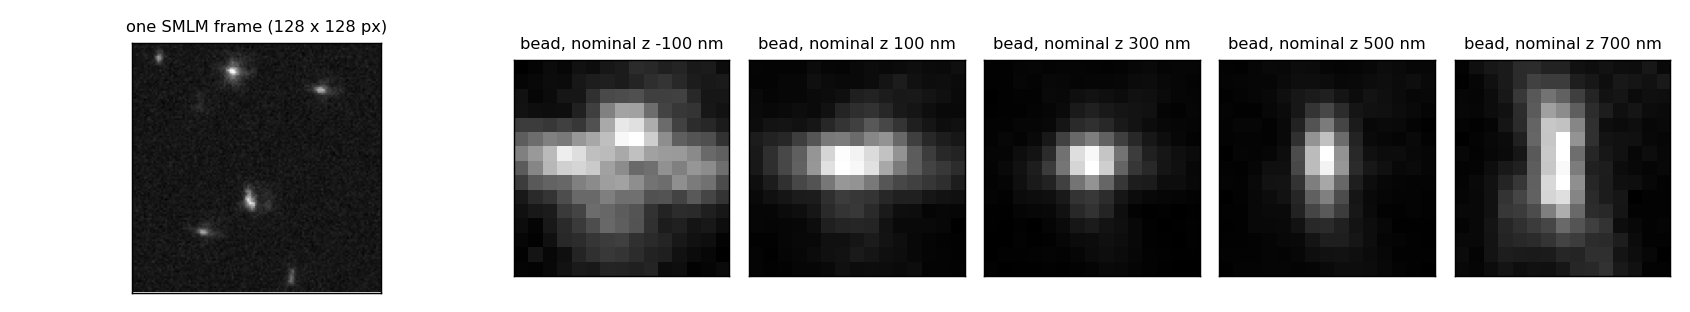
\includegraphics[width=0.95\linewidth]{../fig/data.png}
\caption{Simulated data: bead stack (top) and one frame of the blinking movie.}\end{figure}

Vectorial PSF~\cite{vectorial}: NA 1.49 oil objective ($n=1.518$), sample in water ($n=1.33$), 680\,nm, 108\,nm
pixels, freely rotating dipole, supercritical-angle light included, 0.10 waves of astigmatism, and small random
Zernike aberrations (Noll 5--21).

\begin{itemize}\setlength\itemsep{0pt}
\item \emph{Bead stack}: 6 beads on the coverslip, 26 focus planes 40\,nm apart, 40{,}000 photons per frame.
\item \emph{Movie}: 6000 frames of $128\times128$ pixels, 700 blinking sites at heights 0--800\,nm, fixed focus,
4000 photons per frame (log-normal), background 30 photons per pixel.
\item \emph{Detection}: difference of Gaussians, isolated spots, $15\times15$ patches centred on the peak.
\item \emph{Clean patches}: 11{,}000 isolated emitters simulated directly, without a detection step.
\item \emph{Test set}: 6000 isolated emitters with known positions, heights 50--750\,nm, independent seed.
\item \emph{Bead versus sample}: besides the index mismatch, four aberrations change by 0.02--0.04 waves between
calibration and experiment (Noll 5, 7, 8, 11). The size of this change is a choice, not taken from data.
\item \emph{Scenario A}: the pupil is a Zernike series Noll 5--21, the class of the fitted Zernike model.
\item \emph{Scenario B}: A plus a phase screen of Noll 22--66 (0.06 waves rms) and a patch of the pupil with
60\,\% amplitude loss.
\end{itemize}
The data are generated with a pupil grid of 128 samples and image oversampling 4; the fitted models use a grid
of 64 and oversampling 3, so the simulation is not the fitted model and the structure of scenario B does not lie
on the pixels of the fitted pupil map. All accuracy results are mean $\pm$ standard deviation over \nseeds{}
seeds (new beads, movie, clean patches and test set per seed).

Scoring, on the test set: \emph{likelihood deficit}, the mean extra negative log-likelihood per emitter compared
with the true PSF; \emph{wrong z}, the fraction with a z error above 150\,nm (excluded from the other columns,
and from nothing else); rms errors; \emph{tilt}, the change of the mean error over the 700\,nm z range, from a
straight-line fit of error against true height (for z this is the error of the z scale); and the ratio of
estimated to true photon count.

\begin{figure}[t]\centering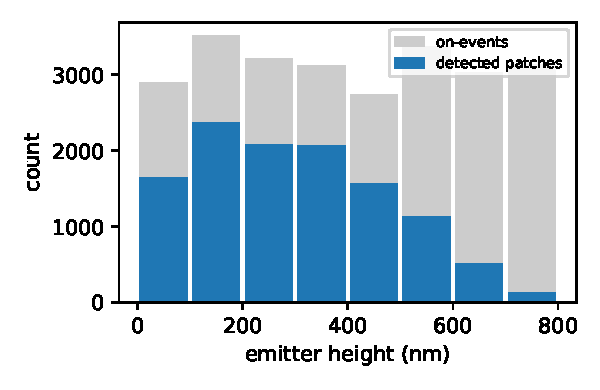
\includegraphics[width=0.45\linewidth]{fig_zhist.pdf}
\caption{On-events of the movie and detected patches against emitter height (scenario A, mean of 3 seeds).}\label{fig:zhist}\end{figure}

Simplifications: Poisson noise only, point-like beads, PSF constant over the field, uniform background, and NA,
refractive indices and wavelength known to the fit.

\section{Results}

\subsection{Speed}
\label{sec:speed}

\begin{table}[t]\centering\small\resizebox{\linewidth}{!}{\begin{tabular}{lrrrrrrrr}\toprule
pupil grid, & model & \multicolumn{3}{c}{per emitter ($\mu$s)} & fixed & break- & \multicolumn{2}{c}{speed-up at $10^4$ / $10^5$ / $10^6$ emitters}\\
oversampling & error & vectorial & spline & localize & (s) & even & gradient & whole iteration\\ \midrule
64, 3 & 0.39\,\% & 10 & 2.3 & 2.5 & 0.006 & 874 & 3.3 / 4.0 / 4 & 2.5 / 2.5 / 2.5\\
128, 4 & 0.15\,\% & 23 & 2.3 & 2.5 & 0.007 & 323 & 7.6 / 9.6 / 10 & 5.0 / 5.2 / 5.3\\
256, 6 & 0.02\,\% & 118 & 2.4 & 2.5 & 0.020 & 171 & 27.1 / 45.8 / 49 & 18.5 / 23.8 / 24.5\\
\bottomrule\end{tabular}}
\caption{Cost of one gradient with respect to the Zernike coefficients (\gpu, \nbench{} emitters measured,
$10^6$ extrapolated linearly). ``Model error'': relative L2 difference of the vectorial model at that setting
from a 256/7 reference. Rates in thousand emitters per second, batches evaluated in parallel. ``Localize'': three Newton steps per emitter on the spline, done in both routes.
``Whole iteration'' includes it.}\label{tab:speed}\end{table}

\begin{figure}[t]\centering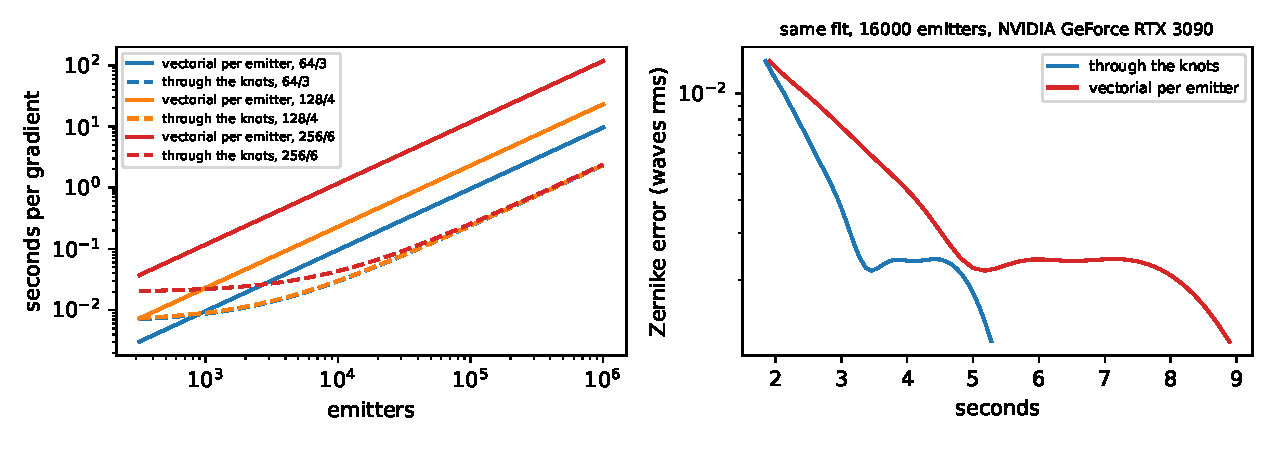
\includegraphics[width=0.95\linewidth]{fig_speed.pdf}
\caption{Left: seconds per gradient against the number of emitters for three settings of the pupil model.
Right: the same fit run with both routes.}\label{fig:speed}\end{figure}

Table~\ref{tab:speed} and Fig.~\ref{fig:speed}. The cost of the pupil model depends on how finely the pupil and
the image are sampled, so each setting is listed with its own numerical error. The spline has an error of
\splineerr\,\%; the setting with a comparable error is 128/4. \speedtext

In both routes the emitter positions are updated on the spline; the comparison is between two ways of getting
the pupil gradient, not against a pipeline that also localizes with the pupil model, which would be slower
still and was not measured. Neither route is optimized beyond batching: the spline gather and scatter are plain
PyTorch autograd, and the pupil model is a matrix Fourier transform in single precision.

\subsection{Is it the same gradient?}
\label{sec:gradacc}

\gradtext

\subsection{Accuracy}

\begin{table}[p]\centering\small
\textbf{Scenario A} (pupil is a Zernike series)\\[2pt]\resizebox{\linewidth}{!}{\begin{tabular}{lrrrrrrr}\toprule
PSF estimate & deficit & wrong $z$ (\%) & $y$ rms & $z$ rms & $y$ tilt & $z$ tilt & $I$ ratio\\
 & (nats) & & (nm) & (nm) & (nm) & (nm) & \\ \midrule
\multicolumn{8}{l}{\emph{patches detected in the movie}}\\
true PSF & 0.00\,$\pm$\,0.00 & 0.1\,$\pm$\,0.0 & 15.4\,$\pm$\,0.2 & 22.4\,$\pm$\,0.3 & 0.8\,$\pm$\,0.4 & -2.1\,$\pm$\,0.1 & 1.00\,$\pm$\,0.00\\
beads only, Zernike & 15.31\,$\pm$\,0.31 & 3.6\,$\pm$\,0.4 & 52.9\,$\pm$\,0.5 & 74.1\,$\pm$\,0.5 & 119.2\,$\pm$\,0.2 & 71.4\,$\pm$\,1.0 & 1.05\,$\pm$\,0.00\\
beads only, spline & 16.93\,$\pm$\,0.71 & 1.6\,$\pm$\,0.4 & 26.2\,$\pm$\,1.3 & 76.1\,$\pm$\,0.5 & 18.5\,$\pm$\,2.7 & -83.4\,$\pm$\,7.2 & 0.73\,$\pm$\,0.00\\
spline shared by beads and movie & 0.22\,$\pm$\,0.04 & 0.3\,$\pm$\,0.1 & 23.6\,$\pm$\,1.4 & 74.0\,$\pm$\,1.3 & 20.6\,$\pm$\,2.8 & -74.9\,$\pm$\,9.5 & 0.73\,$\pm$\,0.00\\
Zernike in situ & 0.02\,$\pm$\,0.00 & 0.1\,$\pm$\,0.0 & 15.4\,$\pm$\,0.2 & 22.4\,$\pm$\,0.4 & -0.9\,$\pm$\,0.8 & -3.1\,$\pm$\,0.5 & 1.00\,$\pm$\,0.00\\
Zernike + free knots & 0.17\,$\pm$\,0.04 & 0.1\,$\pm$\,0.0 & 17.6\,$\pm$\,0.3 & 27.1\,$\pm$\,0.5 & 0.3\,$\pm$\,1.9 & -12.5\,$\pm$\,4.4 & 1.00\,$\pm$\,0.00\\
Zernike + free pupil map & 0.08\,$\pm$\,0.05 & 0.0\,$\pm$\,0.1 & 15.5\,$\pm$\,0.2 & 22.4\,$\pm$\,0.6 & 1.3\,$\pm$\,2.6 & -3.5\,$\pm$\,3.6 & 1.00\,$\pm$\,0.00\\
\multicolumn{8}{l}{\emph{clean patches (no detection step)}}\\
Zernike in situ & 0.01\,$\pm$\,0.00 & 0.1\,$\pm$\,0.0 & 15.4\,$\pm$\,0.1 & 22.4\,$\pm$\,0.4 & -0.1\,$\pm$\,0.6 & -6.2\,$\pm$\,1.1 & 1.00\,$\pm$\,0.00\\
Zernike + free knots & 0.12\,$\pm$\,0.01 & 0.1\,$\pm$\,0.0 & 17.5\,$\pm$\,0.1 & 27.0\,$\pm$\,0.3 & 2.3\,$\pm$\,0.5 & -15.9\,$\pm$\,2.3 & 1.00\,$\pm$\,0.00\\
Zernike + free pupil map & 0.00\,$\pm$\,0.00 & 0.1\,$\pm$\,0.1 & 15.4\,$\pm$\,0.2 & 22.3\,$\pm$\,0.3 & 3.8\,$\pm$\,0.6 & -4.2\,$\pm$\,1.9 & 1.00\,$\pm$\,0.00\\
\bottomrule\end{tabular}}\\[10pt]
\textbf{Scenario B} (pupil has structure outside the Zernike series)\\[2pt]\resizebox{\linewidth}{!}{\begin{tabular}{lrrrrrrr}\toprule
PSF estimate & deficit & wrong $z$ (\%) & $y$ rms & $z$ rms & $y$ tilt & $z$ tilt & $I$ ratio\\
 & (nats) & & (nm) & (nm) & (nm) & (nm) & \\ \midrule
\multicolumn{8}{l}{\emph{patches detected in the movie}}\\
true PSF & 0.00\,$\pm$\,0.00 & 0.1\,$\pm$\,0.0 & 15.1\,$\pm$\,0.1 & 23.0\,$\pm$\,0.2 & 0.8\,$\pm$\,1.0 & -1.5\,$\pm$\,0.5 & 1.00\,$\pm$\,0.00\\
beads only, Zernike & 16.58\,$\pm$\,0.41 & 3.9\,$\pm$\,0.4 & 76.9\,$\pm$\,0.7 & 66.0\,$\pm$\,0.3 & 182.9\,$\pm$\,0.4 & 47.7\,$\pm$\,1.3 & 0.89\,$\pm$\,0.00\\
beads only, spline & 17.89\,$\pm$\,0.34 & 3.8\,$\pm$\,0.6 & 30.1\,$\pm$\,1.1 & 79.7\,$\pm$\,0.5 & 22.2\,$\pm$\,4.5 & -98.0\,$\pm$\,4.9 & 0.62\,$\pm$\,0.00\\
spline shared by beads and movie & 0.32\,$\pm$\,0.02 & 0.7\,$\pm$\,0.2 & 29.7\,$\pm$\,1.8 & 77.2\,$\pm$\,1.1 & 40.5\,$\pm$\,5.8 & -107.0\,$\pm$\,10.1 & 0.62\,$\pm$\,0.00\\
Zernike in situ & 2.75\,$\pm$\,0.09 & 0.1\,$\pm$\,0.1 & 25.0\,$\pm$\,0.3 & 25.7\,$\pm$\,0.6 & 45.3\,$\pm$\,0.7 & 19.0\,$\pm$\,1.9 & 0.85\,$\pm$\,0.00\\
Zernike + free knots & 0.22\,$\pm$\,0.01 & 0.1\,$\pm$\,0.0 & 24.7\,$\pm$\,0.5 & 28.6\,$\pm$\,0.1 & 43.1\,$\pm$\,1.3 & 17.9\,$\pm$\,4.1 & 0.86\,$\pm$\,0.00\\
Zernike + free pupil map & 0.05\,$\pm$\,0.02 & 0.1\,$\pm$\,0.0 & 15.4\,$\pm$\,0.4 & 23.1\,$\pm$\,0.5 & 8.5\,$\pm$\,5.0 & -0.5\,$\pm$\,4.5 & 0.91\,$\pm$\,0.01\\
\multicolumn{8}{l}{\emph{clean patches (no detection step)}}\\
Zernike in situ & 2.66\,$\pm$\,0.09 & 0.1\,$\pm$\,0.1 & 27.5\,$\pm$\,0.5 & 25.1\,$\pm$\,0.3 & 50.9\,$\pm$\,1.0 & 14.1\,$\pm$\,1.0 & 0.85\,$\pm$\,0.00\\
Zernike + free knots & 0.13\,$\pm$\,0.01 & 0.1\,$\pm$\,0.0 & 28.1\,$\pm$\,0.5 & 27.8\,$\pm$\,0.6 & 52.2\,$\pm$\,0.8 & 10.1\,$\pm$\,0.3 & 0.86\,$\pm$\,0.00\\
Zernike + free pupil map & 0.01\,$\pm$\,0.00 & 0.1\,$\pm$\,0.0 & 16.2\,$\pm$\,0.2 & 23.2\,$\pm$\,0.3 & 17.7\,$\pm$\,1.0 & -1.0\,$\pm$\,1.6 & 0.90\,$\pm$\,0.00\\
\bottomrule\end{tabular}}
\caption{PSF estimates scored on the test emitters, mean $\pm$ sd over \nseeds{} seeds.}\label{tab:acc}\end{table}

\begin{figure}[t]\centering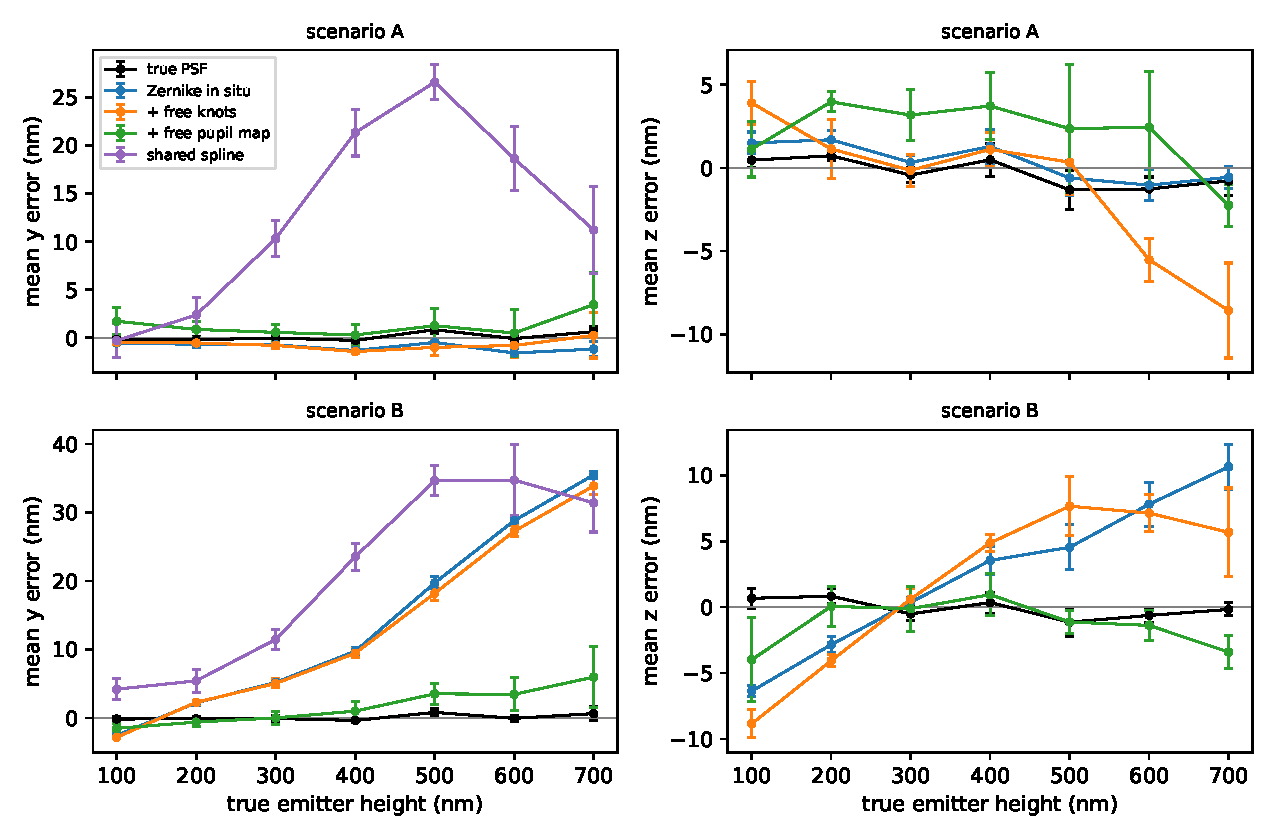
\includegraphics[width=0.9\linewidth]{fig_bias.pdf}
\caption{Mean position error against true emitter height for PSFs estimated from the movie patches. Error bars:
sd over seeds.}\label{fig:bias}\end{figure}

\acctext

\subsection{A pitfall: a limit on the fitted offset}

\pitfalltext

\subsection{An illumination pattern as a second position ruler}

\begin{table}[t]\centering\small\resizebox{\linewidth}{!}{\begin{tabular}{llrrrrrr}\toprule
 & & \multicolumn{3}{c}{with pattern} & \multicolumn{3}{c}{same frames, no pattern}\\
scenario & PSF model & deficit & $y$ range & $z$ range & deficit & $y$ range & $z$ range\\ \midrule
A & Zernike & 0.00 & -0 .. +0 & -4 .. +1 & 0.00 & -0 .. +0 & -5 .. +1\\
A & free pupil map & 0.01 & -0 .. +0 & -2 .. +1 & 0.01 & -1 .. +3 & -1 .. +1\\
A & free knots & 0.12 & -1 .. +1 & -6 .. +2 & 0.16 & -0 .. +1 & -8 .. +2\\
B & Zernike & 2.86 & -3 .. +21 & -4 .. +21 & 2.72 & -2 .. +43 & -7 .. +4\\
B & free pupil map & 0.01 & -1 .. +1 & -3 .. +2 & 0.02 & -3 .. +14 & -2 .. +1\\
B & free knots & 0.21 & -1 .. +2 & -12 .. +21 & 0.29 & -2 .. +44 & -9 .. +4\\
\bottomrule\end{tabular}}
\caption{PSF estimated from emitters seen in 6 frames under a shifting sinusoidal illumination pattern (known
exactly), and from the same frames without pattern. Ranges: smallest and largest mean error over 7 height bins
(nm). One seed.}\label{tab:pattern}\end{table}

\patterntext

\subsection{Real data: nuclear pores}
\label{sec:real}

Data: 3D astigmatic dSTORM of Nup107-SNAP-AF647 in U2OS cells with its bead stack, from the 2016 SMLM
challenge~\cite{challenge} (Ries lab; microscope with a 160$\times$/1.43\,NA objective~\cite{cspline}),
150{,}000 frames of $135\times148$ pixels. The camera pixel size in the sample is not stated in any source we
found; the lateral results below are in pixels or as ratios.

\emph{Bead PSF and first localization.} A free-knot spline was fitted to 30 beads (41 planes, 50\,nm steps,
$\pm800$\,nm; knots every half pixel and 50\,nm; leave-one-bead-out $\chi^2$ per pixel 1.07 against 1.03 in
sample). Localizing the movie with it gives 1.05 million localizations in 240\,s, a median $\chi^2$ per pixel
of 1.00, and a spread between detections of the same emitter in consecutive frames that equals the
Cram\'er--Rao bound (ratio 1.00--1.02; 0.08 pixel laterally, 32\,nm in z). The bead spline therefore already
describes these data well at typical brightness; above 8000 photons the lateral spread is 1.5 times the bound.

\emph{Models compared} (trained on 150{,}000 spots from the even 1000-frame blocks, scored on the 452{,}000
spots of the odd blocks): (a) the bead spline; (b) a vectorial model fitted to the beads (NA 1.43, Zernikes
Noll 5--36, radial apodization, pixel size fitted); (c) as b with the Zernikes refined on the movie through the
knots; (d) as c plus free pupil phase and amplitude maps; (e) free knots refined on the movie, starting from
the bead spline.

\begin{table}[t]\centering\small
\begin{tabular}{lrrrrr}\toprule
 & a & b & c & d & e\\
 & bead & bead & Zernike & c + pupil & free knots\\
 & spline & vectorial & in situ & maps & in situ\\ \midrule
deviance per spot relative to a & 0 & $-0.50$ & $-1.21$ & $-1.74$ & $-2.55$\\
repeat z spread (nm, in the z units of a) & 32.1 & 31.7 & 31.5 & 31.2 & 36.0\\
same, above 8000 photons & 12.4 & 13.7 & 13.9 & 12.6 & 8.6\\
repeat x spread (pixel) & 0.0848 & 0.0845 & 0.0841 & 0.0840 & 0.0848\\
z spread within a pore (nm, in the z units of a) & 32.9 & 32.6 & 32.6 & 32.2 & 35.5\\
two Nup107 rings resolved & no & no & no & no & no\\
ring radius relative to a & 1 & 1.0005 & 1.0019 & 1.0022 & 1.0040\\
z scale relative to a & 1 & 1.03 & 1.11 & 1.10 & 0.98\\
largest z-dependent lateral shift relative to a (nm) & -- & 14 & 37 & 33 & 2\\ \bottomrule
\end{tabular}
\caption{Nuclear-pore data, held-out frames. Deviance: twice the negative log-likelihood difference per
$17\times17$ pixel spot, lower is better (standard errors 0.005 to 0.011). Repeat spread: robust spread between
detections of the same emitter in consecutive frames, divided by $\sqrt2$ (338{,}636 pairs, the same pairs for
all methods). The z values of each method were converted to the z axis of the bead spline with the local slope
before comparing. Within-pore spread: 5063 pore clusters, each centred per 3000-frame window to remove drift.
Lateral shift in nm with the fitted pixel size of model b.}\label{tab:real}
\end{table}

Table~\ref{tab:real}.
\begin{itemize}\setlength\itemsep{0pt}
\item \emph{Likelihood.} Refining the vectorial model in situ gives a real held-out gain over the bead spline
($-1.2$ per spot for the Zernikes, $-1.7$ with pupil maps), and over the bead vectorial model it started from.
\item \emph{Precision.} The gain in z precision is 3\,\% at most (d), and nothing changes laterally. No method
resolves the two rings of Nup107, which are about 50\,nm apart in z.
\item \emph{Geometry.} The in-situ vectorial models (c, d) stretch the z axis by about 10\,\% relative to the
bead spline and add z-dependent lateral shifts of up to 35\,nm. Which geometry is right cannot be decided from
these data: there is no independent ruler for z, and the ring radius changes by only 0.2\,\%.
\item \emph{Free knots} (e) reach the best likelihood but a worse z precision (36 against 32\,nm), their
Cram\'er--Rao bound for z (19.5\,nm) is far below the observed spread, and their geometry stays that of the
bead spline (z scale 0.98, lateral shift 2\,nm). This is the behaviour predicted in section~\ref{sec:gauge}
and seen in the simulation. Only for the brightest emitters do they give the smallest spread.
\item \emph{The vectorial model does not fit the beads as well as a spline} ($\chi^2$ per pixel 1.20 against
1.06), with the misfit in the core of the PSF in defocused planes. The bead data exclude an NA of 1.46 or
higher but do not separate NA, wavelength and pixel size from each other.
\item \emph{Speed.} One iteration of fit c with 150{,}000 emitters took 1.9\,s, of which 89\,\% was
re-localization and 0.2\,s the gradient through the knots (GPU shared with other jobs). The fit had converged
after about 50 iterations.
\end{itemize}
So on this data set the in-situ vectorial refinement is fast and improves the fit of the images, but a bead
spline was already at the Cram\'er--Rao bound, and the practical gain is small. The open question it raises is
the z scale, which needs a sample with known axial structure.

\subsection{Real data: microtubules}
\label{sec:tub}

Data: 3D astigmatic dSTORM of microtubules (AF647) from the same challenge and microscope, 4 movies with
10.1 million bead-spline localizations of which 6.7 million pass the quality flags, and a bead stack of 401
planes with only 7 usable beads, all in the lower half of the field. The stage step is not documented; we
assume 10\,nm. A microtubule is a cylinder, so its cross-section should be round. This gives a check on the z
scale that the nuclear pores did not: the ratio of lateral to axial width of the cross-section, $\kappa$, is
the factor by which the z axis of a method must be multiplied to make it round. Li et al.~\cite{cspline} use
0.75 for the refractive index mismatch.

The models a to e and the split in frame blocks are as in section~\ref{sec:real} (150{,}000 training spots,
3.35 million test spots, 1.74 million consecutive-frame pairs). The settings of d and e (roughness penalty,
number of iterations) were chosen on a separate validation set of 30{,}000 spots.

\emph{Ruler.} 33 straight, isolated 1\,$\mu$m microtubule segments (108{,}823 spots) were selected on the image
of method a; segments with a second filament nearby were dropped. Drift, which is not corrected in these data,
was fitted as one shift per 2000 frames shared by all segments. The width of the cross-section is the observed
spread minus the localization precision (Cram\'er--Rao bound times the repeat ratio of that brightness class)
in quadrature. Uncertainties are from a bootstrap over segments.

\begin{table}[t]\centering\small
\begin{tabular}{lrrrrr}\toprule
 & a & b & c & d & e\\
 & bead & bead & Zernike & c + pupil & free knots\\
 & spline & vectorial & in situ & maps & in situ\\ \midrule
deviance per spot relative to a & 0 & $+0.86$ & $-0.35$ & $-1.73$ & $-10.2$\\
repeat x spread (pixel) & 0.0922 & 0.0935 & 0.0939 & 0.0941 & 0.0924\\
repeat z spread (nm, in the z units of a) & 27.2 & 27.4 & 27.7 & 27.7 & 21.3\\
same, above 8000 photons & 19.7 & 19.9 & 20.4 & 20.5 & 11.0\\
z scale relative to a & 1 & 1.03 & 1.11 & 1.17 & 1.02$^*$\\
largest z-dependent lateral shift relative to a (nm) & -- & 20 & 42 & 33 & 28\\
$\kappa$ from the microtubule cross-section & 0.74 & 0.71 & 0.68 & 0.65 & 0.34\\
\quad 95\,\% interval & 0.62--0.92 & 0.60--0.86 & 0.58--0.80 & 0.55--0.79 & 0.28--0.43\\ \bottomrule
\end{tabular}
\caption{Microtubule data, held-out frames; rows as in Table~\ref{tab:real} (standard errors of the deviance
0.002 to 0.02). $\kappa$: lateral width of the microtubule cross-section divided by its axial width in the z
units of that method; a correct z axis has $\kappa=1$, and an axis that still needs the index-mismatch factor
has $\kappa\approx0.75$. Lateral values use a pixel size of 117.6\,nm. $^*$The z axis of e is strongly warped
(local slope between 0.1 and 1.4), so one scale factor does not describe it.}\label{tab:tub}
\end{table}

\begin{figure}[t]\centering
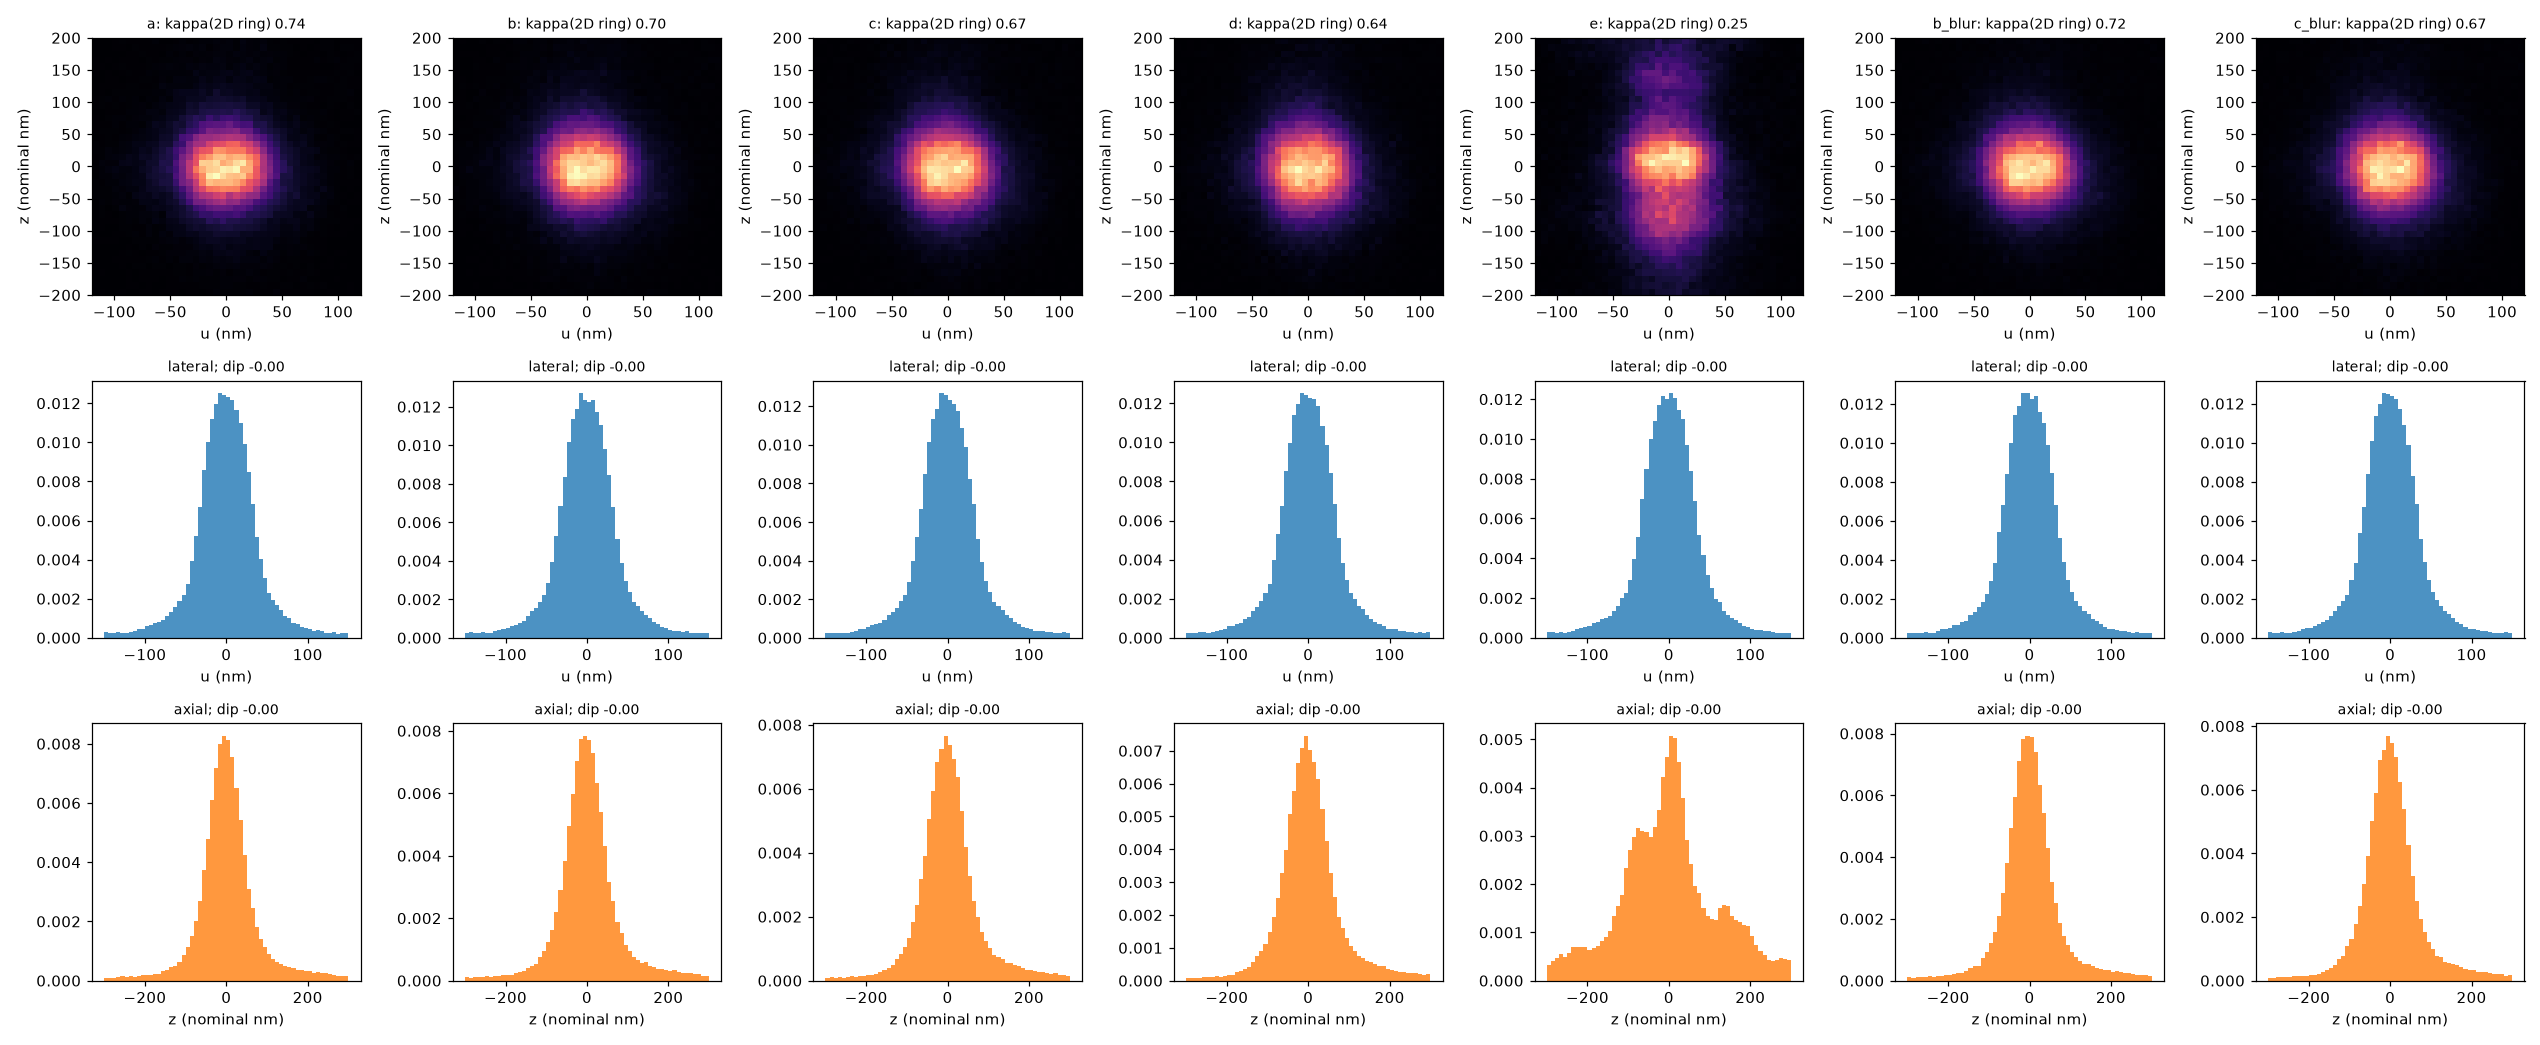
\includegraphics[width=\textwidth]{fig_tub_profiles.png}
\caption{Microtubule cross-sections pooled over 33 segments, for the bead spline (a), bead vectorial model (b),
Zernikes refined in situ (c), with pupil maps (d), free knots (e), and b and c with an added Gaussian blur.
Top: density across the filament (u) and along z; middle and bottom: lateral and axial profiles. The free knots
(e) spread the filament over several peaks in z.}\label{fig:tub}
\end{figure}

Table~\ref{tab:tub} and Fig.~\ref{fig:tub}.
\begin{itemize}\setlength\itemsep{0pt}
\item \emph{The vectorial model fits these beads poorly} ($\chi^2$ per pixel 9.4 against 3.0 for the spline;
on the nuclear-pore beads 1.20 against 1.06). The misfit is in the core of the PSF at all z. Adding a Gaussian
blur of 50\,nm brings it to 7.4, free pupil maps to 5.8, both to 3.9. The single-molecule fit asks for the
same blur (54\,nm), so it is not the bead size (100\,nm beads would give about 22\,nm); its cause is unknown.
As a result the bead vectorial model (b) is worse than the bead spline on the movie ($+0.86$).
\item \emph{Likelihood.} Refining in situ recovers this and ends below the bead spline: $-0.35$ for the
Zernikes, $-1.73$ with pupil maps. The gain grows with brightness ($-15$ per spot above 8000 photons for d).
\item \emph{Precision.} None of the vectorial models improves the repeat spread; it becomes 1 to 2\,\% worse in
both x and z. The lateral spread of bright spots stays far above the Cram\'er--Rao bound for all methods
(ratio 3.0 above 8000 photons for a).
\item \emph{Geometry.} As on the nuclear pores, the in-situ vectorial models stretch z relative to the bead
spline, by 11\,\% (c) and 17\,\% (d), with lateral shifts of up to 42\,nm.
\item \emph{The ruler does not decide the z scale.} For the bead spline $\kappa=0.74$ (0.62--0.92), which
agrees with 0.75. The values for b, c and d differ from it only by their z scale and lie inside each other's
intervals. The ruler is also not clean: $\kappa$ depends on brightness (0.87 for spots below 1500 photons, 0.62
at 1500--3000, about 0.37 at 3000--6000, because the axial width rises with brightness while the lateral width
does not) and is not monotonic in depth. Bright spots therefore carry z errors that persist over consecutive
frames; overlapping emitters along the filament are a possible cause, not shown. The hollow core of the
microtubule is not resolved by any method.
\item \emph{Free knots look best and are wrong.} Model e has by far the best likelihood ($-10.2$) and repeat
z spread (21 against 27\,nm; 11 against 20\,nm for bright spots). On the ruler its cross-section is 78\,nm wide
in z against 36\,nm for the bead spline, with several peaks ($\kappa=0.34$). Its z axis is warped; between
$-600$ and $-400$\,nm it has almost no z sensitivity left. A stiffer version (ten times less deviance gain,
nearly linear z) is still wider than the bead spline (43\,nm). So free knots on blinking data give z values
that repeat from frame to frame but are wrong per emitter, and neither the held-out likelihood nor the repeat
precision detects this. This is the gauge freedom of section~\ref{sec:gauge} on real data.
\item \emph{Speed.} As on the nuclear pores: 1.9\,s per iteration of fit c for 150{,}000 emitters, 89\,\%
re-localization, 0.19\,s for the gradient through the knots (shared GPU).
\end{itemize}
Taken together, the two data sets show an in-situ vectorial refinement that is fast and improves the fit of the
images, but no measurable gain in localization quality over a bead spline, and a 10 to 17\,\% difference in
z scale that neither data set can assign to one of the two. What the microtubules add is a warning: held-out
likelihood and repeat precision can both improve while the positions get worse, so a PSF refined in situ needs
a check against known structure.

\section{Relation to other methods}

\begin{itemize}\setlength\itemsep{1pt}
\item INSPR~\cite{inspr}, VISPR~\cite{vispr}: z classes, averaging, phase retrieval on the averages. The route
here is the exact-likelihood counterpart of this pooling (section 2.3).
\item uiPSF~\cite{uipsf}: automatic differentiation and L-BFGS over PSF and emitter parameters, with the pupil
model evaluated per emitter; its voxel PSF is offered for bead data only.
\item Droste et al.~\cite{droste}: alternating maximum likelihood with field-dependent Zernike coefficients,
1000--5000 emitters; the optical transfer function is precomputed on patches of the field, a saving over the
field that is similar in spirit to the saving over emitters here.
\item Spline and lookup-table localization~\cite{cspline,hauser}: tabulated PSFs, not used to learn the pupil.
\end{itemize}
To our knowledge no published in-situ method back-propagates the likelihood through a tabulated PSF to a pupil
model. The literature search behind this statement was made from preprints and code repositories and was not
exhaustive.

For a field-constant Zernike PSF a few thousand emitters suffice, and at that size the route has no advantage.
It matters where many emitters are needed: a pupil map with thousands of free pixels, aberrations that vary
over the field or in time, and very large data sets. None of these is demonstrated here.

\section{Limitations}

\limittext

\begin{thebibliography}{9}\small
\bibitem{inspr} F. Xu et al., Three-dimensional nanoscopy of whole cells and tissues with in situ point spread
function retrieval, Nat. Methods 17, 531 (2020).
\bibitem{vispr} H. Yang et al., VISPR: in situ vectorial PSF retrieval, Photonics Research (2024),
doi:10.1364/PRJ.520469.
\bibitem{uipsf} S. Liu et al., Universal inverse modeling of point spread functions for SMLM accurately predicts
their complex aberrations, Nat. Methods 21 (2024), doi:10.1038/s41592-024-02282-x.
\bibitem{droste} I. Droste et al., vectorial in-situ PSF fitting with field-dependent aberrations, Optica (2025);
bioRxiv 2024.12.11.627909.
\bibitem{cspline} Y. Li et al., Real-time 3D single-molecule localization using experimental point spread
functions, Nat. Methods 15, 367 (2018).
\bibitem{babcock} H. P. Babcock and X. Zhuang, Analyzing single molecule localization microscopy data using
cubic splines, Sci. Rep. 7, 552 (2017), doi:10.1038/s41598-017-00622-w.
\bibitem{challenge} D. Sage et al., Super-resolution fight club: assessment of 2D and 3D single-molecule
localization microscopy software, Nat. Methods 16, 387 (2019).
\bibitem{hauser} F. Hauser and J. Jacak, lookup-table based 3D localization (2021), PMC8407837.
\bibitem{vectorial} S. Stallinga and B. Rieger, Accuracy of the Gaussian point spread function model in 2D
localization microscopy, Opt. Express 18, 24461 (2010).
\end{thebibliography}
References are not yet checked against the published versions (titles of \cite{vispr,droste,hauser} are
descriptive placeholders).
\end{document}
